\chapter{Kravspecifikation}


\section{Versionshistorik}
\begin{longtabu} to \linewidth{@{}l l l X[l]@{}}
    Version 	&    Dato 		&    Ansvarlig 	&    Beskrivelse\\[-1ex]
    \midrule
    0.1 		&  	21-09-2015 	&   MHNK og MBA 	&   Oprettelse og udfyldning af kravspecifikation \\
	0.2			&	24-09-2015	&	DHC og ABH	&	Omskrivning af UC1 - UC5 \\
	0.3			&	28-09-2015	&	ABH			&	Ikke-funktionelle krav \\
	0.4			&	08-10-2015	&	Alle		&	Tilrette efter review med Grp. 1 \\
	0.5			&	15-10-2015	&	MBA			&	Indskrevet i LaTex \\
	0.6			&	11-11-2015	&	ABH			&	Ændre Use Case 1 og 2 efter review med Grp. 4 \\
	0.7			&	20-10-2015	&	MHNK		&	Tilretning \\
	0.8			&	26-11-2015	&	MHNK		&	Retning af hele kravspec. \\
	0.9			&	09-12-2015	&	DHC			&   Rettelser ift. software \\
	1.0			&	09-12-2015	&	MHNK		&   Rettelse af afsnit i rapport og dokumentation \\  
    
\label{version_Systemark}
\end{longtabu}

\section{Godkendelsesformular}
\begin{longtabu} to \linewidth{@{}l X[j]@{}}
	Forfattere	&	Anne Hoelgaard, Ditte Heebøll Callesen, Martin Banasik, Albert Fredshavn, Mathias Munk og Mette Hammer Nielsen-Kudsk \\
	\midrule
	Godkendes af & Peter Johansen \\
	Antal sider & \pageref{LastPage} \\
	Kunde	&	IHA \\
\end{longtabu}

Ved underskrivelse af dette dokument accepteres det af begge parter, som værende kravene til udviklingen af det ønskede system.
\\
\\
\\
\\
\noindent \begin{tabular}{lll} 
	& 	\makebox[2.5in]{\hrulefill} 	& 	\makebox[2.5in]{\hrulefill}\\
	&	Sted						&	Dato\\[7ex]
	& 	\makebox[2.5in]{\hrulefill} 	& 	\makebox[2.5in]{\hrulefill}\\
	& 	Kundens underskrift 		& 	Leverandørens underskrift\\[7ex]

\end{tabular}
\section{Indledning}
På baggrund af krav fra kunden samt, hvad leverandøren finder muligt, er denne kravspecifikation blevet udarbejdet. Kravspecifikation har til formål at specificere kravene til produktet. Dette projekt tager udgangspunkt i en blodtryksmåler, hvortil der er en række aktører, som interagerer med systemet, der er beskrevet yderligere nedenfor.

\section{Systembeskrivelse}
Blodtryksmålersystemet ønskes udviklet således at systolisk og diastolisk blodtryk samt puls kan bestemmes ud fra en invasiv ateriel blodtryksmåling. Der udvikles instrumentering til den udleverede transducer som hardware og et software-program til kontinuerligt visning af målt blodtryk, samt til udskrivelse af løbende systoliske, diastoliske og puls værdier. Disse to dele udgør til sammen systemet. 

\section{Funktionelle krav}
 

\subsection{Aktør-kontekstdiagram}


\begin{figure}[H]
	\centering
	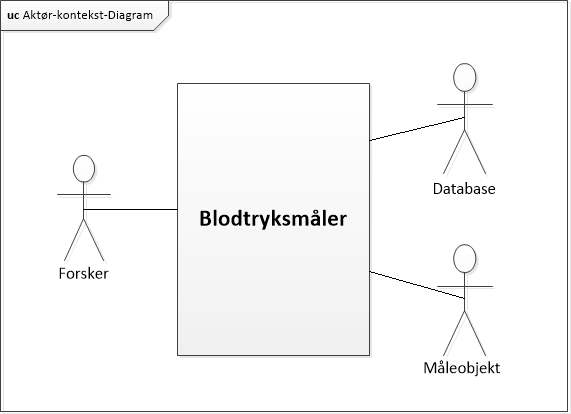
\includegraphics[width=0.8\textwidth]{Figurer/Aktor-kontekst-diagram}
	\caption{Aktør-kontekstdiagram}
	\label{fig:aktoerbeskrivelse}
\end{figure}
På figur \ref{fig:aktoerbeskrivelse} ses aktørerne til at være: Forsker, Måleobjekt og Database. Herunder er der en detaljeret beskrivelse af hver aktør.


\subsection{Aktørbeskrivelse}

\begin{table}[H]
\begin{tabularx}{\textwidth}{l l X}
     Aktørnavn	&	Type		&	Beskrivelse \\ \midrule
     Forsker   	& 	Primær  	& 	Forskeren er aktøren, der starter måling, giver besked om at data ønskes gemt, navngiver målingen samt afslutter måling af blodtryk \\ 			  \addlinespace[2mm]
     Database	&	Sekundær	&	Databasen er aktøren, hvori måledata bliver gemt \\   \addlinespace[2mm]
     Måleobjekt	&	Sekundær	&	Måleobjekt er aktøren, hvorfra blodtrykssignalet indhentes. Måleobjektet er tilkoblet transduceren
     I den endelige version er måleobjektet In Vitro maskinen, som findes i Cave Lab
     Under løbende test i udviklingsprocessen benyttes Analog Discovery og Waveform \\   \addlinespace[2mm]
     
   
     \bottomrule                                                                                                                   
    \end{tabularx}
    \caption {Aktørbeskrivelse}
    \label{tab:aktoerbeskrivelse}
	
\end{table}

\subsection{Use case-diagram}

\begin{figure}[H]
	\centering
	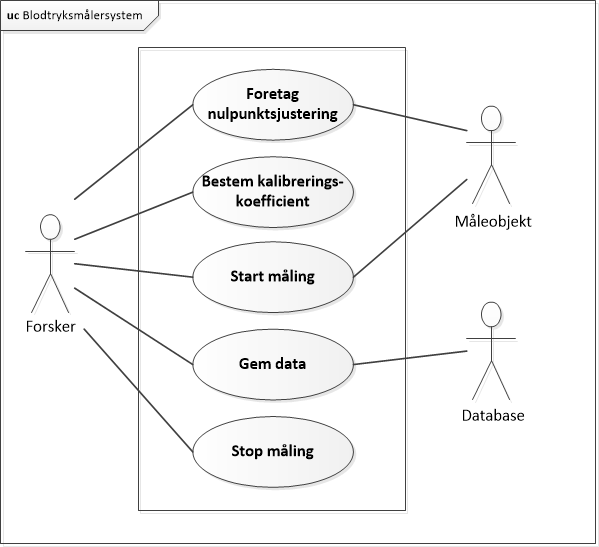
\includegraphics[width=0.8\textwidth]{Figurer/UseCasediagram}
	\caption{Use Case-diagram}
	\label{fig:Use Cases}
\end{figure}

Diagrammet ovenfor viser systemets fem Use Cases: Foretag nulpunktsjustering, Foretag kalibrering, Start måling, Gem data og Afslut måling. Herunder følger en nærmere beskrivelse af de enkelte Use Cases, gennem et fully-dressed Use Case skema. \\
\newline
Systemet består af en computer, hvor softwaren er placeret, en NI-DAQ, en Analog Discovery samt en transducer med tilhørende implementering. Systemet gør det muligt at foretage en blodtryksmåling på et måleobjekt, som er tilsluttet og sender disse signaldata ind i systemet via transduceren og det tilhørende hardware, hvor signalet vises. Det ønskede interval af blodtrykssignalet gemmes så i databasen. \\
I softwaren benyttes algoritmer til at analysere signalet, ud fra opsatte grænseværdier, så systolisk, diastolisk og puls værdier hentes frem. Disse algoritmer undersøger signalet for, hvor signalets bølgetoppe og -bunde er placeret. Da top er signalets systoliske værdi og bund er signalets diastoliske. Puls bestemmes ved at tælle antallet af blodtryksperioder pr. minut. \\    
Brugergrænseflade er det, som forsker initierer med, altså hvorfra systemet aktiveres. Brugergrænsefladen forkortes til GUI. 

\subsection{Use Cases}

\begin{longtabu} to \linewidth{@{}l r X[l]@{}} %UC1%
	{\large \textbf{Use Case 1}} && \\
	\toprule
	Scenarie 				&&	Hovedscenarie\\
	Navn 					&& 	Foretag nulpunktsjustering\\
	Mål 					&& 	At få foretaget en nulpunktsjustering\\
	Initiering 				&& 	Startes af Forsker\\
	Aktører 				&& 	Forsker (primær), Måleobjekt (sekundær)\\
	Referencer 				&& 	\\
	Samtidige forekomster  	&& 	Én nulpunktsjustering pr. kørsel \\
	Forudsætninger 			&&	Alle systemer er ledige og operationelle\\ 
	Resultat 				&& 	Nulpunktsjustering er blevet fortaget efter ønske\\ \midrule
	Hovedscenarie 			&    1. 	&	Pop-up vindue for nulpunktsjustering er åbent\\				 	
							&    2. 	& 	Forsker trykker på:\\ 
							& 			&	a. Ja-knap for at starte en nulpunktsjustering\\[-1ex]
							& 			&		 i. System beder om udlignelse af atmosfærisk tryk\\[-1ex]
							& 			&		 ii. System venter på bekræftigelse fra forsker\\[-1ex]
							& 			&		 iii. Nulpunktsjustering foretages og vinduet lukker efter endt justering\\[-1ex]
							& 			&  	b. Nej-knap for ikke at få foretaget en nulpunktsjustering\\[-1ex]
							& 			&   ii. Vinduet lukker\\[-1ex]	
	Undtagelser 			&			& 	-  \\ \bottomrule
	
	\caption{Fully dressed Use Case 1}
	\label{UC1}
\end{longtabu}

\begin{longtabu} to \linewidth{@{}l r X[l]@{}} %UC2%
	{\large \textbf{Use Case 2}} && \\
	\toprule
	Scenarie && Hovedscenarie\\
	Navn && Foretag kalibrering\\
	Mål && At få foretaget et valg om kalibrering, samt evt. udført kalibrering\\
	Initiering && Startes af Forsker\\
	Aktører && Forsker (primær), Måleobjekt (sekundær)\\
	Referencer && Use Case 1\\
	Samtidige forekomster  && Én kalibrering pr. kørsel \\
	Forudsætninger && Alle systemer er ledige og operationelle\\ 
	Resultat && Kalibrering er blevet foretaget efter ønske \\ \midrule
	Hovedscenarie &    1. &		Pop-up vindue for kalibrering er åbent\\				 	
	&    2. & Forsker trykker på:\\ 
	& &	a. Ja-knap for at starte en kalibrering\\[-1ex]
	& &		 i. System beder om signal til justering\\[-1ex]
	& &		 ii. System venter på bekræftigelse fra forsker\\[-1ex]
	& & 	 iii. Kalibrering foretages og vinduet lukker efter endt kalibrering\\[-1ex]
	& &  b. Nej-knap for ikke at få foretaget en kalibrering\\[-1ex]
	& &   ii. Vinduet lukker\\[-1ex]	
	Undtagelser && -  \\ \bottomrule
	
	\caption{Fully dressed Use Case 2}
	\label{UC2}
\end{longtabu}

\begin{longtabu} to \linewidth{@{}l r X[l]@{}} %UC3%
    {\large \textbf{Use Case 3}} && \\
    \toprule
    Scenarie && Hovedscenarie\\
    Navn && Start Måling\\
    Mål && At få foretaget en blodtryksmåling\\
    Initiering && Startes af Forsker\\
    Aktører && Forsker (primær), Måleobjekt (sekundær)\\
    Referencer && Use Case 1 og Use Case 2\\
    Samtidige forekomster  && Ét signal pr. måling\\
    Forudsætninger && Use Case 1 og Use Case 2 er kørt succesfuldt, samt alle systemer kører og er klar til at foretage en måling\\ 
    Resultat && Systolisk-, diastolisk blodtryk samt puls bliver vist på GUI\\ \midrule
    Hovedscenarie &    1. &		Forsker indtaster Forsøgsnavn\\[-1ex]
    &     2. & 	Filteret signal er valgt per default af systemet\\	 	
                &    & [\textit{Undtagelse 1:}] Forsker vælger ufiltreret signal på radiobutton	\\
                &    3. & Forsker trykker på Start-knap på GUI\\[-1ex]
                &    4. & Signal for blodtryk vises på GUI\\[-1ex] 
                &    5. & Systolisk og diastolisk blodtryk samt puls bliver vist i bokse på GUI\\ \midrule
                
    Undtagelser && [\textit{Undtagelse 1}]	Forsker vælger ufiltreret signal\\ 
    &	a. & Use Case fortsættes fra punkt 3\\ 
    \bottomrule
\caption{Fully dressed Use Case 3}
\label{UC3}
\end{longtabu}


\begin{longtabu} to \linewidth{@{}l r X[l]@{}} %UC4%
    {\large \textbf{Use Case 4}} && \\
    \toprule
    Scenarie && Hovedscenarie\\
    Navn && Gem data\\
    Mål && At gemme data i databasen\\
    Initiering && Startes af Forsker\\
    Aktører && Forsker (primær), Database(sekundær)\\
    Referencer && Use Case 1 - 3 \\
    Samtidige forekomster  &&  Ét signal pr. måling\\
    Forudsætninger && Use Case 1 og 2 er kørt succesfuldt, Use Case 3 kører. VPN er tilsluttet\\
    Resultat && Systolisk- og diastolisk blodtryk samt puls er blevet gemt i en Database under Forsøgsnavn\\ \midrule
    Hovedscenarie &    1. &		Forsker trykker på Gem-knap\\[-1ex] 
    &	2. & Systemet gemmer det fremadrettede ufiltreret signal i Database\\
                  &    3. &  Forsker trykker på Gem-knap for at stoppe med at gemme\\
    &	&			[\textit{Undtagelse 1:}] Forsker trykker på Afslut-knap\\
                    &    4. &   Det fremgår af GUI at data er gemt\\ \midrule	 	
 Undtagelser &    & [\textit{Undtagelse 1:}] Forsker trykker på Afslut-knap\\
 & a. 	&  Systemet stopper med at gemme, hvorefter systemet lukker\\  

 \\ \bottomrule
\caption{Fully dressed Use Case 4}
\label{UC4}
\end{longtabu}

\begin{longtabu} to \linewidth{@{}l r X[l]@{}} %UC5%
	{\large \textbf{Use Case 5}} && \\
	\toprule
	Scenarie && Hovedscenarie\\
	Navn && Afslut måling \\
	Mål && At stoppe måling af blodtryk\\
	Initiering && Startes af Forsker\\
	Aktører && Forsker (primær)\\
	Referencer && Use Case 1 -3  \\
	Samtidige forekomster  &&  Ét signal pr. måling\\
	Forudsætninger && Use Case 1 og 2 er kørt succesfuldt, Use Case 3 kører\\
	Resultat && Måling af blevet stoppet\\ \midrule
	Hovedscenarie &    1. &		Forsker trykker på Afslut-knap\\[-1ex] 
	&    2. &   Måling stopper, hvorefter systemet lukker \\ \midrule	 	
	Undtagelser &    & - 	\\ \bottomrule
	\caption{Fully dressed Use Case 5}
	\label{UC5}
\end{longtabu}

\section{Ikke-funktionelle krav}


\subsection{(F)URPS+}

\textbf{Functionality}
\begin{enumerate}
\item Blodtryksmåleren skal indeholde en Start-knap til at igangsætte målingerne. 
\item Blodtryksmåleren skal indeholde en Afslut-knap, hvorfra måling kan stoppes.
\item Blodtryksmåleren skal indeholde en Gem-knap til at gemme målingerne i Databasen.
\item Blodtryksmåleren skal indeholde en tekstboks til forsøgsnavn, hvori forsker indtaster det pågældende forsøgsnavn.
\item Blodtryksmåleren skal indeholde radiobutton til filtreret signal, denne skal være default valget.
\item Blodtryksmåleren skal indeholde radiobutton til ufiltreret signal.
\item Blodtryksmåleren skal indeholde tekstbokse til puls, systolisk og diastolisk blodtryk som vises med op til tre cifre.
\item Blodtryksmåleren skal indeholde en tekstboks som viser filnavn på målingen, mens målingen foretages. 
\item GUI’en skal se ud som vist på figur \ref{fig:Skitse af GUI}:
\begin{figure}[H]
	\centering
	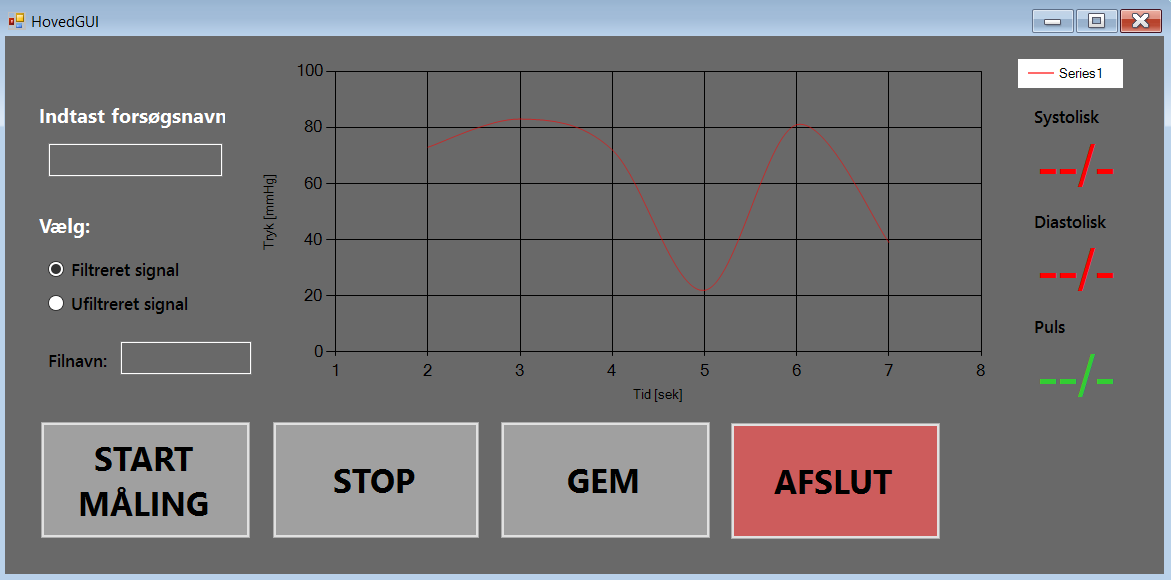
\includegraphics[width=0.8\textwidth]{Figurer/GUI}
	\caption{Skitse af GUI}
	\label{fig:Skitse af GUI}
\end{figure}

\end{enumerate}

\textbf{Usability}
\begin{enumerate}
\item Forskeren skal kunne starte en default-måling maksimalt 30 sekunder efter systemet er startet.
\end{enumerate}

\textbf{Reliability}
\begin{enumerate}
\item Det skal maksimalt tage 5 timer at gendanne systemet (MTTR - Mean Time To Restore)
\item Systemet skal have en oppetid uden nedbrud på minimum 1 måned (720 timer) (MTBF - Mean Time Between Failure).   
\item Systemet skal have en oppetid/køretid på: 
\end{enumerate}

				\begin{align}
					Availability = \frac{MTBF}{MTBF+MTTR}\cdot100 = \frac{720}{720+5}\cdot100 = 99,31 \%
				\end{align}



\textbf{Performance}
\begin{enumerate}
\item Blodtryksmåleren skal, indenfor 3 sekunder, kunne vise systolisk og diastolisk blodtryk via graf. Dette accepteres med en tolerance på +/- 15 \%.
\item Blodtryksmåleren skal, inden for måleperioden, kunne alarmere hvis måleobjekt har forhøjet eller for lavt blodtryk. Defineres efter grænseværdier beskrevet i… xxxx…
\item Blodtryksmåleren skal, indenfor 30 sekunder fra der er trykket på Gem-knap, kunne gemme målingerne i Databasen.  Dette accepteres med en tolerance på +/- 15 \%.
\item Grafen vises i ét vindue, hvor y-aksen måles i mmHg (millimeter kviksølv) og x-aksen i tid pr. sekund. 
\item Hvert 7. sekund skal værdier for systolisk og diastolisk blodtryk samt puls opdateres. Dette accepteres med en tolerance på +/- 15 \%.
\item Graf for blodtryk skal køre kontinuerligt i GUI efter følgende princip(figur \ref{fig:Graf for blodtryks visning}), hvor det blå signal erstatter det orange signal ved at den seneste måling altid sættes ved cursorens placering.
\begin{figure}[H]
	\centering
	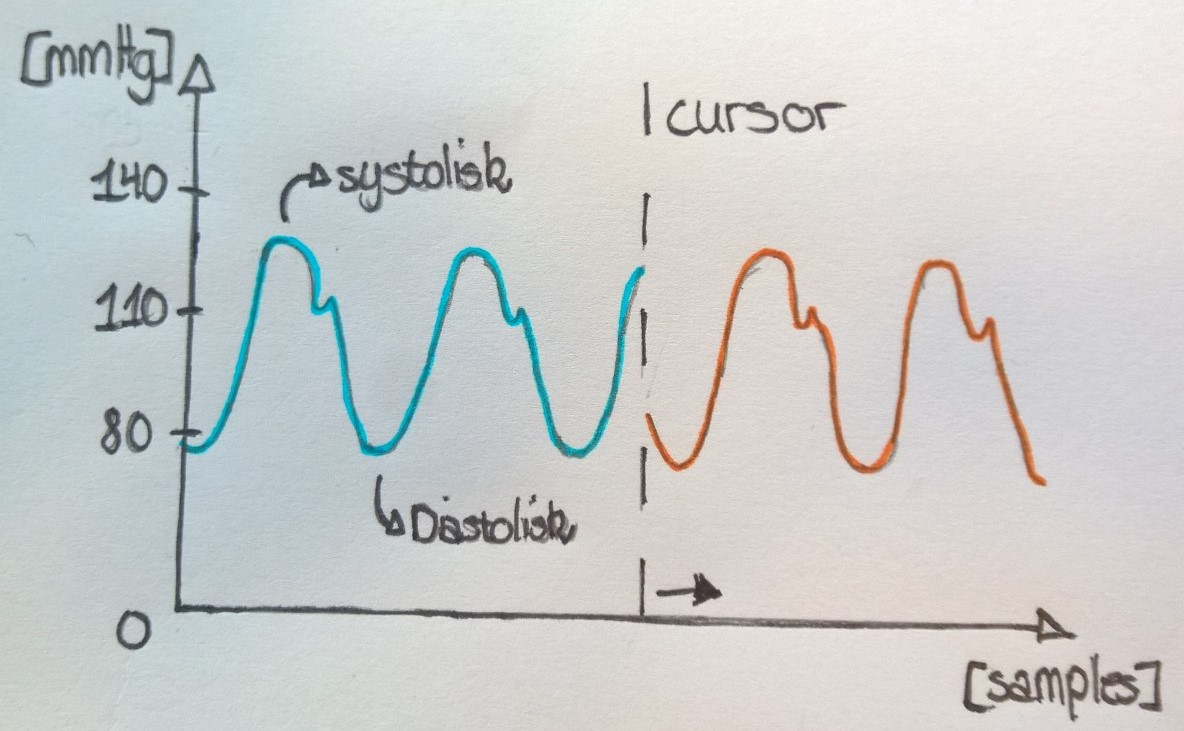
\includegraphics[width=0.6\textwidth]{Figurer/Cursor}
	\caption{Graf for blodtryk}
	\label{fig:Graf for blodtryks visning}
\end{figure}

\item Når der trykkes på Gem-knap gemmes det ufiltrerede signal under det indtastede forsøgsnavn og et autogenereret id. \textit{"forsøgsnavn\_id"}.
\item Systemet skal kunne måle blodtryksværdier fra 0 til 250 mmHg.
\end{enumerate}


\textbf{Supportability}
\begin{enumerate}
\item Forskeren skal kunne udskifte hardwaren på 10 minutter. 
\item Softwaren skal opbygges med lav kobling. 
\end{enumerate}
















